\documentclass[paper=a4, fontsize=11pt]{scrartcl}

\usepackage[bottom=2em]{geometry}


\usepackage{amssymb}
\usepackage{tikz}
\usepackage{hyperref}
\usepackage{graphicx}
\hypersetup{colorlinks=true}
%\graphicspath{ {/home/sergiu/work/rc/part2part/rapport/} }



\title{Part2Part}
\author{Iacob Sergiu B1}
\date{\normalsize\today}

\begin{document}

\maketitle

\newpage

\section{Introduction}

\paragraph{}
Part2Part is a peer-to-peer application meant to satisfy a user's need of sharing documents with colleagues. The facilities which this project brings are meant for anyone who wishes to transfer files with ease.
Any user connected to this platform is able to share multiple files from his local storage and gives access to other users to them so they can acquire them as well.

\section{Technologies}
\paragraph{}
The protocol used for communicating between the clients and the server is UDP. As this protocol does not ensure the safe retrieval of every sent package (as TCP would do), the application manually does this by hash-verifying every package.
The application also consists of an attractive web server, which users will use to easily browse through the available files for download, as well as sharing them.

\section{Architecture}
\paragraph{}
As this is a peer-to-peer application, each user will act as both a client and a server. The main server will filter all of the commands, the main ones being $GetFile(file X, from B)$ and $SendFile (file X, to B)$.
\paragraph{}
The core of the Part2Part application consists in file sharing between users. When a certain user A executes a $GetFile(file X, from B)$ command, where B is a user whose file X is available for download, the user A will shortly have to his disposal the requested file. 

\paragraph{}
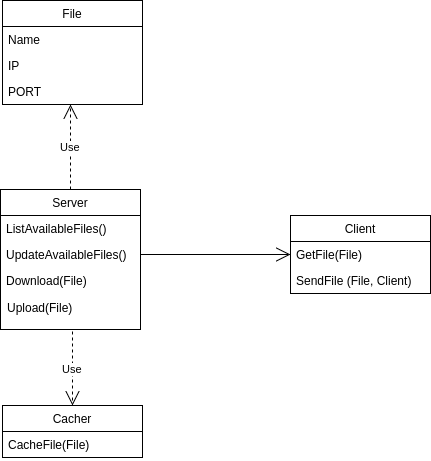
\includegraphics[width=270px]{diagram.png}

\newpage

\section{Implementation details}
\paragraph{}
The server is built using C++. The user interface is built using HTML and JavaScript.
\paragraph{}
The first step a user takes is to connect to the server. The server is implemented in a concurret manner and will assign a different thread for the newly connected user, so that it may serve each individual simultaneously.
\paragraph{}
After connecting, the user will be able to search for files based on their name as it follows:
\begin{itemize}  
\item Search files after name
\item The server checks if any documents with that name are available from the connected users
\item Receive a list of available items for download
\end{itemize}
He may now choose a file to download, but he may be prompted for a password to acquire the document.
\paragraph{}
Another service the user might use is putting at disposal documents from his local storage as it follows:
\begin{itemize}  
\item Enter file name
\item The server updates its database with the name, ip and port at which the file may be found
\item The server will assign to the ip and to the port 2 strings, for ease of use
\item The file is now available for download
\item The file may be downloaded by another user by specifying its name, the ip and port (as strings) from which was uploaded on the server
\end{itemize}

The server also uses a local file cacher, so that it will work faster. The latest and most asked for documents will be locally stored, for faster transfers.

\section{Conclusions}
\paragraph{}
Part2Part represents a solution that provides a hassle-free experience in sharing documents on a simple platform. It also represents a good example for various use-cases for UDP and the disadvantages this protocol has, as well as the incredible facilities the Internet is offering us.

\section{Bibliography}

\begin{itemize}  
\item \href{https://profs.info.uaic.ro/~computernetworks/index.php}{Computer Networks}
\item Stack	 Overflow
\end{itemize}
\end{document}